\section{研究内容与技术路线}

本课题拟实现一个基于法条的判案论点细粒度挖掘的司法辅助系统,
本论文的工作分为如下几个方面,如\cref{fig_1}所示。
该系统首先细粒度解耦法律条文,
根据法律条文获得分析案件所需的维度。
在此基础上,以案情描述作为输入,基于细粒度解耦的法律条文,
自动挖掘判案论点并且自动识别案情描述中的关键信息。
最后,根据判案论点和案情描述中的关键信息,
分析论证每一个判案论点所需的证据,
预测该案件判决为某罪名所需的完备证据集。
上述三个功能组合成完整的司法辅助系统,
从而能够辅助司法从业者分析理解与决策。
\begin{figure}[h]
	\centering
	% 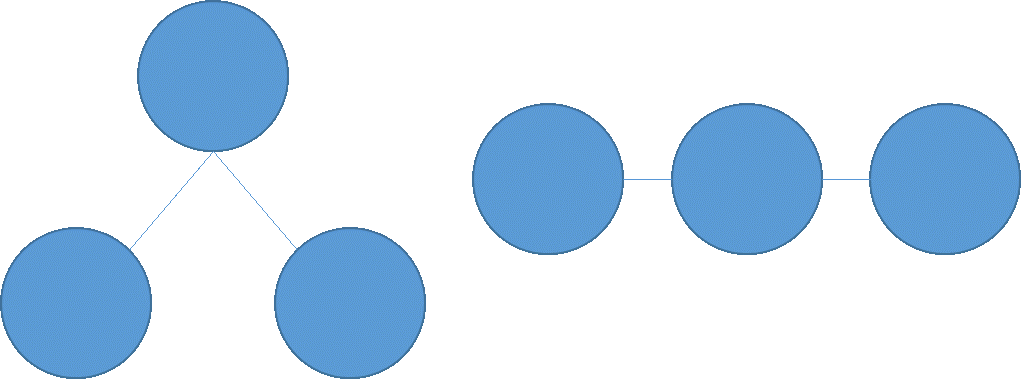
\includegraphics[width=0.4\linewidth]{fig_1.png}

	\scriptsize
	\tikzstyle{format}=[rectangle,draw,fill=white,font=\fontsize{12pt}{18pt}\selectfont]
	\begin{tikzpicture}
		\node[format] (law){法律条文细粒度解耦};
		\node[format,right of=law,node distance=45mm] (argument){判案论点挖掘};
		\node[format,right of=argument,node distance=45mm] (key_info){案情描述关键信息识别};
		\node[format,below of=argument,node distance=15mm] (evidence){完备证据集预测};
		\node[format,below of=key_info,node distance=15mm] (legal){司法下游任务};
		\draw[->] (law)--(argument);
		\draw[->] (argument)--(key_info);
		\draw[->] (argument)--(evidence);
		\draw[->] (key_info)--(evidence);
		\draw[->] (key_info)--(legal);
		% \draw[->](setkeycheck)--node[above]{Yes}(setsetflag);
		% \draw[->](setkeycheck) --node[left]{No} (readtime);
	\end{tikzpicture}
	\caption{研究内容关系示意图}
	\label{fig_1}
\end{figure}

\subsection{研究内容一:法律条文细粒度解耦}
根据现有的司法法律条文,我们从法律条文中细粒度解耦出分析案件所需的维度。
法律条文的内容具有一定的抽象性、概括性、精确性和整体性。
从学理上将,中国是典型的大陆法系国家,
大陆法系要求法官遵从法律明文办理案件,
这与英美法系的判例法有着明显的区别。
所以,辅助国内司法从业者,
就需要对法条进行细粒度解耦,
并根据解耦的要素来指导进一步对案情描述的分析。

\textbf{\color{red} 此处贴法律条文细粒度解耦的举例图}

\subsection{研究内容二:判案论点挖掘}
对于一篇给定的案情描述,
我们拟基于法律条文解耦得到的重要维度,
自动总结出该案件的判案论点。
之后,根据每一个判案论点,
从案情描述中自动识别出对应关键信息,
将法律条文与案情描述进行论点上的关联和维度上的对应。
这一部分的判案论点和关键信息可以被使用于罪名预测、法条预测等司法下游任务,
该种方式不仅具有更强的可解释性,
而且能够更好的辅助司法从业人员理解案情、书写文书以及做出决策。

\textbf{\color{red} 此处贴判案论点挖掘的举例图}

\subsection{研究内容三:司法证据预测与生成}
在司法案件中,完备的证据集至关重要,
其在定罪与量刑中起着决定性的作用。
所以根据一个案件的案情描述,总结出其完备的证据集,
能够很好的辅助到司法从业者。
我们拟基于案情描述的文本信息以及上述挖掘的判案论点,
根据每一个论点预测生成对应证据,
列举完备的论据可以充分论证判案论点,
从而构建出完备的证据集。

\begin{figure}[h]
	\centering
	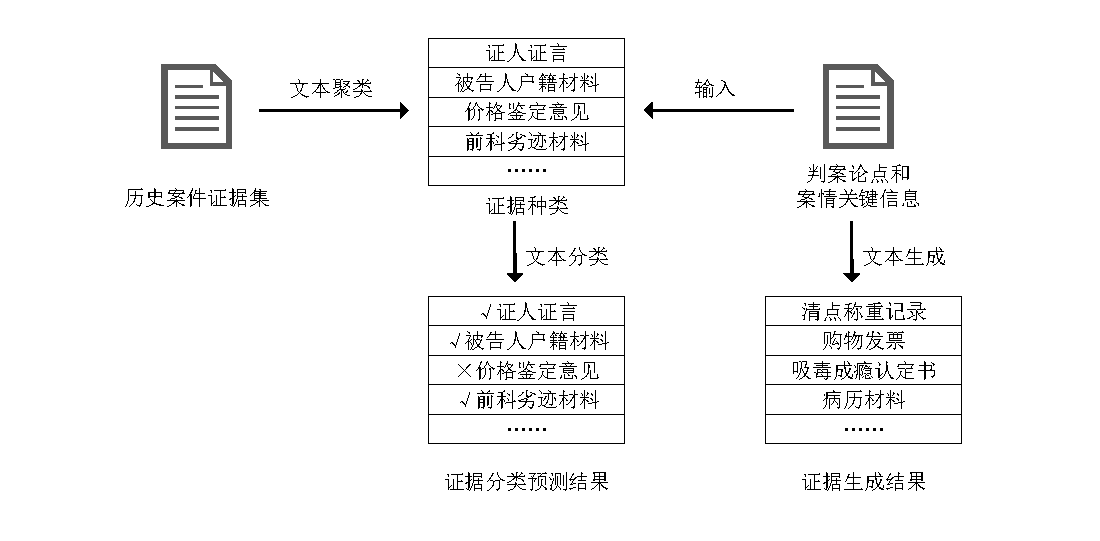
\includegraphics[width=0.8\linewidth]{evidence_generation.pdf}
	\caption{司法证据预测与生成任务说明}
	\label{evidence}
\end{figure}

如\cref{evidence}所示,
对于案情描述,
其包含的证据一部分的作用为论证
该案情所涉及的法条所解耦出的维度。
另一部分的作用为证明案情中描述的某一特定事实,
这一部分的证据往往不能通过聚类汇聚成一个证据类别,
而是根据案情描述的具体内容进行生成。
因此,本工作拟对这两种证据分别进行生成。


\subsection{基于注意力机制和强化学习的判案论点挖掘}

由于司法领域的独特性,
模型给定的司法预测结果都需要具有可解释性。
因为中国使用的是大陆法系,
所以司法从业人员做出的决策都是遵从的法律明文,
故而,模型在给定任何司法预测结果前,
都需要基于法条内容,
给出该案情描述所对应的判案论点和包含的关键信息。
此处,本工作拟使用注意力机制和强化学习共同完成该任务。

在判案论点挖掘中,
为了更好的体现语义高度凝练法律条文的指导作用,
本工作拟通过注意力机制指导案情描述的文本进行解读。
具体来说,如\cref{attention}所示,
本工作拟使用法律条文解耦出的维度信息作为查询,
来指导模型关注到案情描述中的最相关的语义文本。
从而,能够分辨出案情描述中的关键信息,
忽略掉在法条指导下不相关、不重要的语义信息,
实现判案论点挖掘。
此时挖掘的判案论点和注意力机制下所关注到的文本片段,
可以辅助完成其他司法任务,并且提供可解释性。

\begin{figure}[h]
	\centering
	\begin{tikzpicture}[semithick]
		\node[draw,inner sep=0.3cm,on grid,label=left: similarty](similarty) {$\alpha$};
		\node[below of=similarty,draw, circle,inner sep=0.2cm,node distance=1.5cm,label=below: fact](k) {K};
		\node[above of=similarty,draw, circle,inner sep=0.2cm,fill=gray!50,node distance=1.5cm,on grid,label=above:law](q) {Q};
		\node[right of=similarty,draw,inner sep=0.3cm,node distance=2cm,on grid,label=below: softmax](scale) {$\beta$};
		\node[right of=scale,draw,inner sep=0.3cm,node distance=2cm,on grid](multiply) {*};
		\node[below of=multiply,draw, circle,inner sep=0.2cm,node distance=1.5cm,on grid,label=below:fact](v) {V};
		\node[right of=multiply,draw,inner sep=0.3cm,node distance=2cm,on grid,label=below: attention](attention) {$A$};
		
		\draw [->](k)--(similarty);
		\draw [->](q)--(similarty);
		\draw [->](similarty)--(scale);
		\draw [->](scale)--(multiply);
		\draw [->](multiply)--(attention);
		\draw [->](v)--(multiply);
	\end{tikzpicture}
	\caption{基于注意力机制的判案论点挖掘}
	\label{attention}
\end{figure}

具体的计算过程如下。
其中A即为基于法律条文计算出的案情描述的注意力值。
$$ \alpha = Q_{law} K^{T}_{fact} $$
$$ \beta  = softmax(\frac{\alpha}{\sqrt{d_k}}) $$
$$ A  = \beta * V_{fact} $$

对于案情描述中的关键信息抽取,
本工作期待通过注意力机制得到的文本是可读的。
因此,本工作引入了强化学习机制,
以罪名预测等司法任务的结果作为激励,
最终让模型能够在每一个案情描述的文本片段上做出
是否为关键信息的二元决策。

\subsection{基于文本聚类的司法证据关联和预测}
针对司法证据,
本工作首先构造了一个司法证据的数据集,
数据集包括案情描述、该案件证据集、罪名、所用法条和处罚结果。
本工作为关联组织来自不同案件、论证不同判案论点的分散证据,
选择使用InfoMap算法\upcite{rosvall2008maps},将证据视为短文本,
进行文本的无监督聚类。

本工作使用SimBERTv2模型,
将证据文本向量化。
之后InfoMap算法将SimBERTv2模型转换为的文本向量,
通过最小化熵来寻求最优的证据文本聚类结果。
之后,将聚类结果中出现频次较多的类别归堆,
关联后视为同一种证据,
在之后,基于案情描述预测证据集的任务时,
将会使用关联总结后的证据类别进行预测。

\textbf{\color{red} 此处贴InfoMap算法的简单原理公式和图}

\subsection{基于序列到序列模型的司法证据生成}
在一部分的案情描述中,
有一部分的证据来自于案情描述的具体需求。
例如:案情描述中提及了“嫌疑人通话”的内容,
那么本案件就需要“通话记录”作为证据之一。
所以,这一部分的司法证据,
则需要根据案情描述的具体文本进行生成。

因为,本工作使用序列到序列模型,
来完成这部分的司法证据生成。
该序列到序列模型的输入为,
案情描述的片段,
输出则为证明该片段所需的证据。
如果该段案情描述无需额外特殊证据证明,
则不进行输出。

\begin{figure}[h]
	\centering
	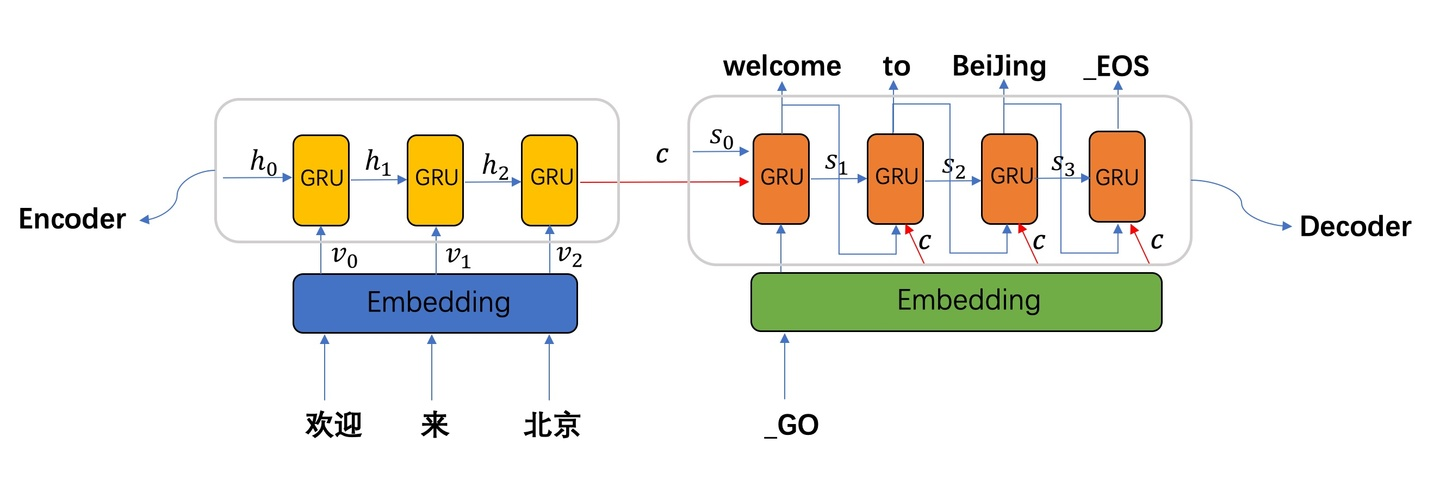
\includegraphics[width=0.8\linewidth]{seq2seq.jpg}
	\caption{序列到序列模型}
	\label{seq}
\end{figure}

序列到序列学习(Seq2Seq)指的是训练模型学习从一个序列到另一个序列的映射函数。
Seq2Seq模型通常都是基于编码器-解码器的架构,
分为编码器(Encoder)和解码器(Decoder)两部分,
其结构如\cref{seq}所示。
其中Encoder需要接收、处理输入序列,
并且编码生成对应的上下文向量,
作为下一步的语境;
而Decoder会接收上一步产生的上下文向量,
逐步预测目标序列的下一个字符,
从而完成全部目标序列的生成。